\section{Results}
\label{sec:results}

Figure \ref{fig:beta} shows a Hovmöller-diagram of a planetary Rossby wave in the northern hemisphere mid-latitudes. We can see that the wave propagates westward with a eastward group velocity, consistent with eqs. \eqref{eq:phasespeed} and \eqref{eq:groupvelocity} without a zonal mean flow.
	\begin{figure}[htbp]
		\centering
		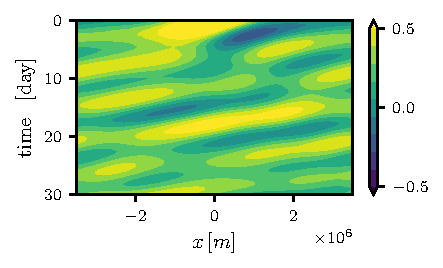
\includegraphics{beta}
		\caption{Hovmöller-diagram showing wave propagation at $y=0$ for 30 days at $45^\circ \,$ N with a planetary vorticity gradient $\beta \equiv 1.66 \cdot 10^{-11} \,$ s.}
		\label{fig:beta}
	\end{figure}

Exploring the effect of topography, Figure \ref{fig:topo} shows the effect of sloping topography. Opposite to what is shown in Figure \ref{fig:topo} the wave propagates eastward with a westward group velocity.
	\begin{figure}[htbp]
		\centering
		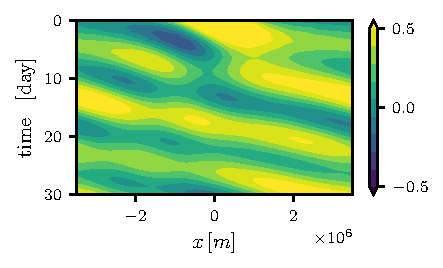
\includegraphics{topo}
		\caption{Hovmöller-diagram showing wave propagation at $y=0$ for 30 days at $45^\circ \,$ N with a planetary vorticity gradient $\beta \equiv 0 \,$ s and topography $\alpha = - 4.46 \cdot 10^{-4}$.}
		\label{fig:topo}
	\end{figure}

With the demonstrated effect of topography, a balance between topography and the planetary vorticity gradient may be obtained, as shown in Figure \ref{fig:compensation} where the Rossby wave is arrested at the same location throughout the entire 30 day period. This is the case for $\alpha = -6.64 \cdot 10^{-4}$, which is the analytical value as calculated from eq. \eqref{eq:dispersion}.
	\begin{figure}[htbp]
		\centering
		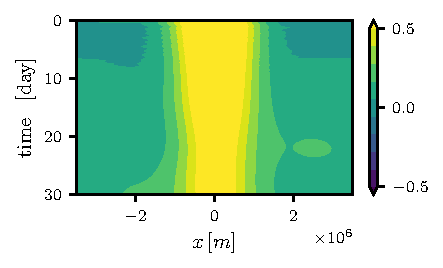
\includegraphics{compensation}
		\caption{Hovmöller-diagram showing wave propagation at $y=0$ for 30 days at $45^\circ \,$ N with a planetary vorticity gradient $\beta \equiv 1.66 \cdot 10^{-11} \,$ s and topography $\alpha = -6.64 \cdot 10^{-4}$.}
		\label{fig:compensation}
	\end{figure}

As a baseline comparison with theory (solid lines), the zonal group (blue) and phase (orange) velocities of planetary waves were estimated numerically (dots) as shown in Figure \ref{eq:phasespeed}. There is a large discrepancy in group velocity for $kR \approx 1$ and phase velocity for $kR \approx 2$.
	\begin{figure}[htbp]
		\centering
		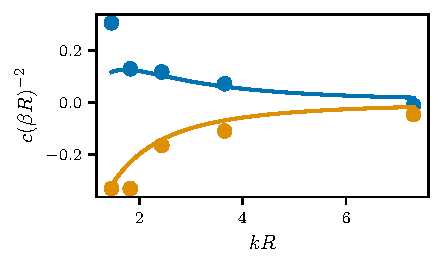
\includegraphics{velocities}
		\caption{Group (blue) and phase (orange) velocities of planetary waves calculated from a Hovmöller diagram as a function of wavenumber. Points - numerical values and lines - analytical values.}
		\label{fig:velocities}
	\end{figure}

The effect of a eastward mean flow is demonstrated in Figure \ref{fig:groupvelocities} where the zonal group velocity is shown as a function of zonal mean flow. The black line shows the analytical dependence, while the grey line is fitted to the numerically calculated points. All numerical values slightly overestimate the analytical values. Extrapolating linear dependence yields zero group velocity for a westward mean flow $U_0 \approx -5\, \text{m}\text{s}^{-1}$.
	\begin{figure}[htbp]
		\centering
		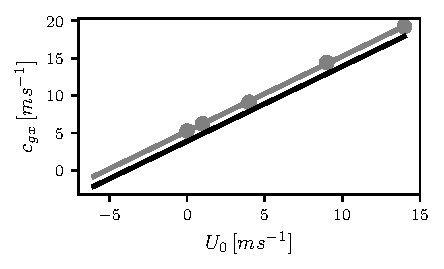
\includegraphics{group_velocities}
		\caption{Group velocities of planetary waves as a function of zonal mean flow. Grey - numerical values with linear fit $c = 5.24 + 1.00 x$ and black - analytical values.}
		\label{fig:groupvelocities}
	\end{figure}